%--------------------------------------------------------
%--------------------------------------------------------
\subsection{Application to Planck 353 Ghz polarization maps}
In this section we apply the local convolution estimator for E and B mode maps on Planck 353 GHz polarization data. To work with out local convolution method, we reduce the resolution of the map to $Nside=128$ using the Healpix \textit {ud\_grade} function. We use a high pass filters which retains modes in the multipole range $\ell=[50,256]$. The non-locality parameter given $\ell_{\rm max}=256$ is $\beta_o=17^{\circ}$. We estimate the local E and B mode maps by performing local convolutions for a set of radial cut-offs: $r_{\rm cutoff} = \beta_o, 0.5\beta_o, 0.25\beta_o$. We do not use any mask while carrying out this analysis. The resultant E and B mode maps are depicted in \fig{fig:353ghz-eb-maps}.
%
\begin{figure}[!h] 
\centering
\subfigure[]{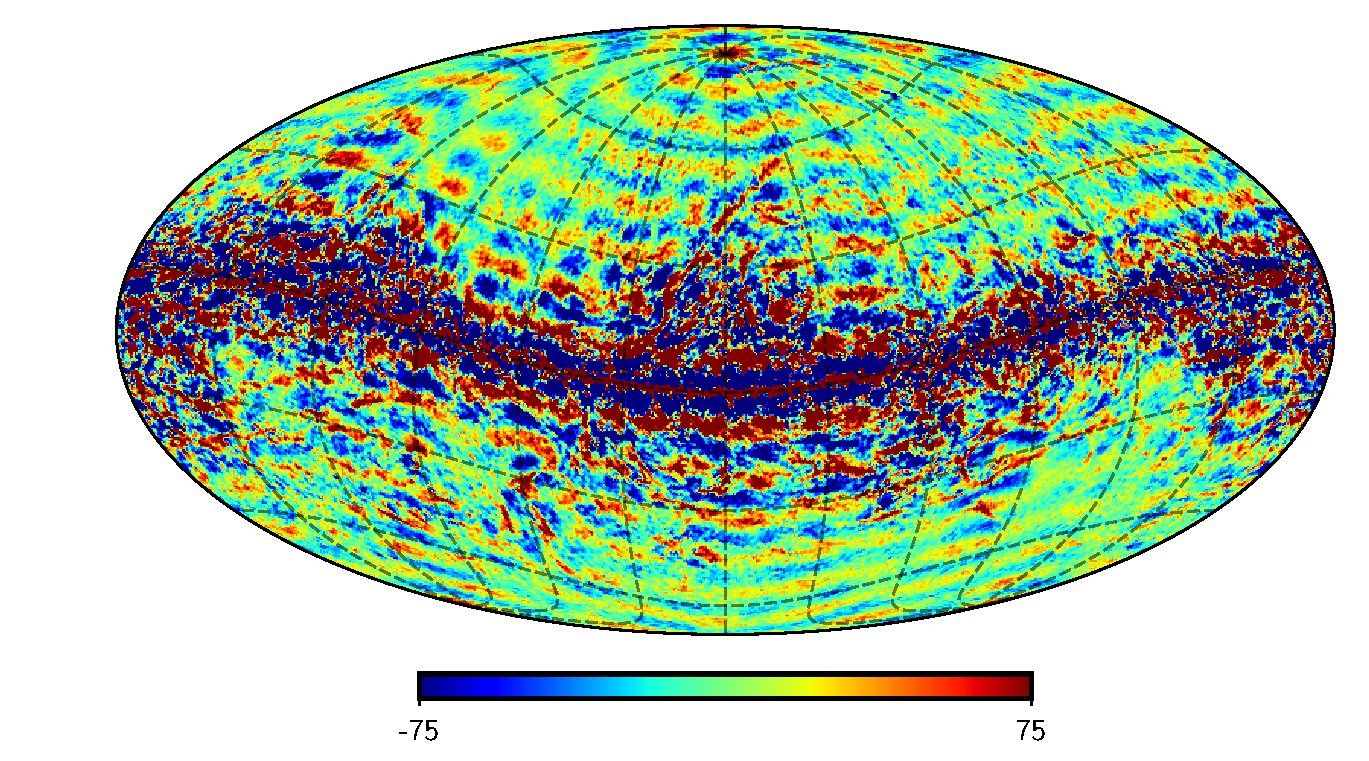
\includegraphics[width=0.49\columnwidth]{353ghz/353ghz-e-mode-healpix_filter_lmin30_lmax256_nside128.pdf}}
\subfigure[]{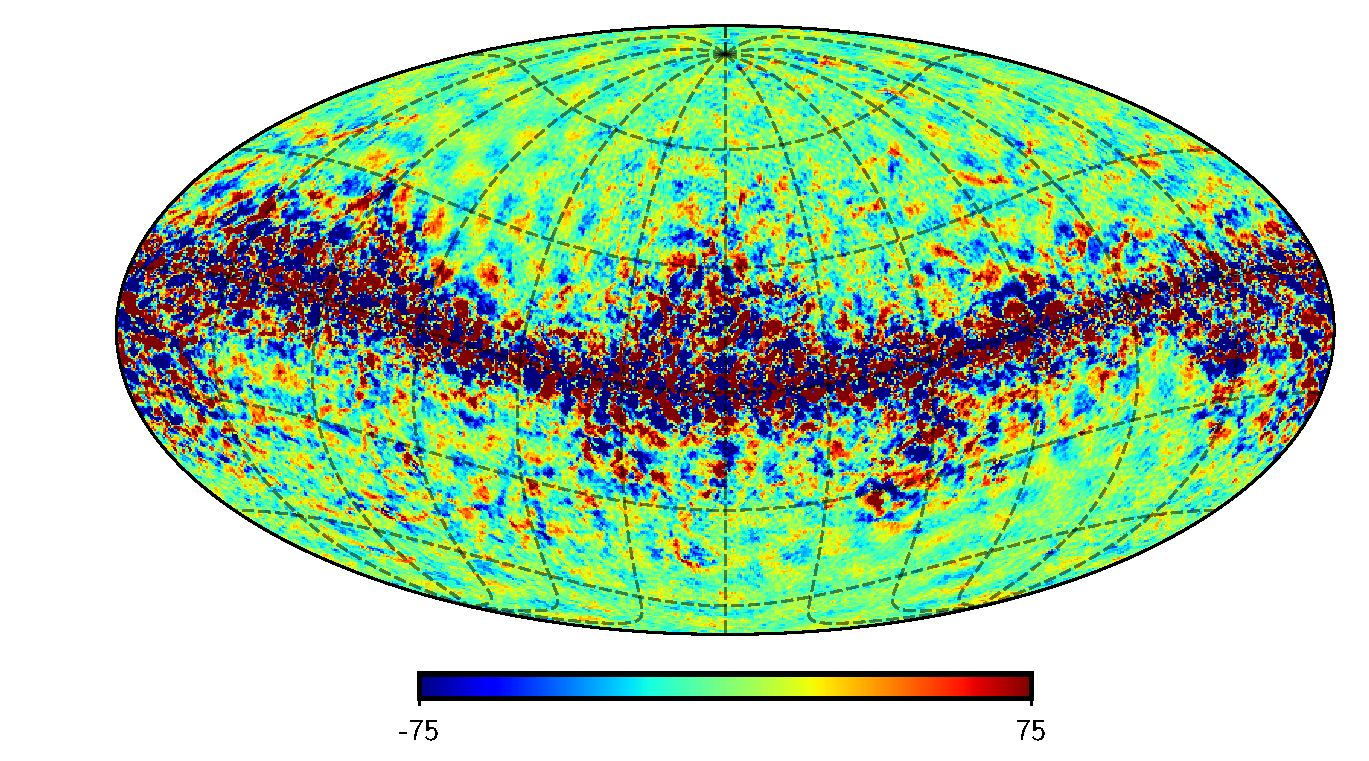
\includegraphics[width=0.49\columnwidth]{353ghz/353ghz-b-mode-healpix_filter_lmin30_lmax256_nside128.pdf}}
\subfigure[]{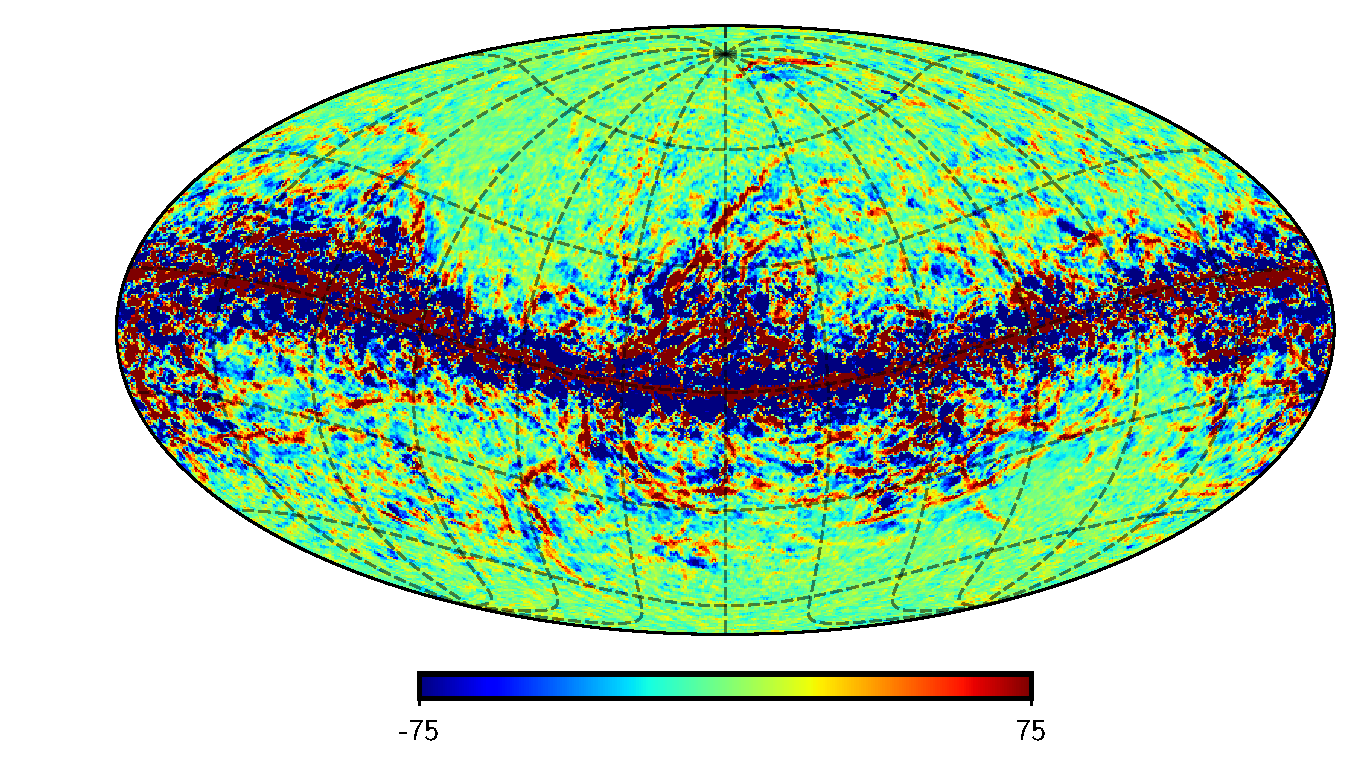
\includegraphics[width=0.49\columnwidth]{353ghz/353ghz-e-mode-realspace_disc7d_apo0d_lmin30_lmax256_nside128.pdf}}
\subfigure[]{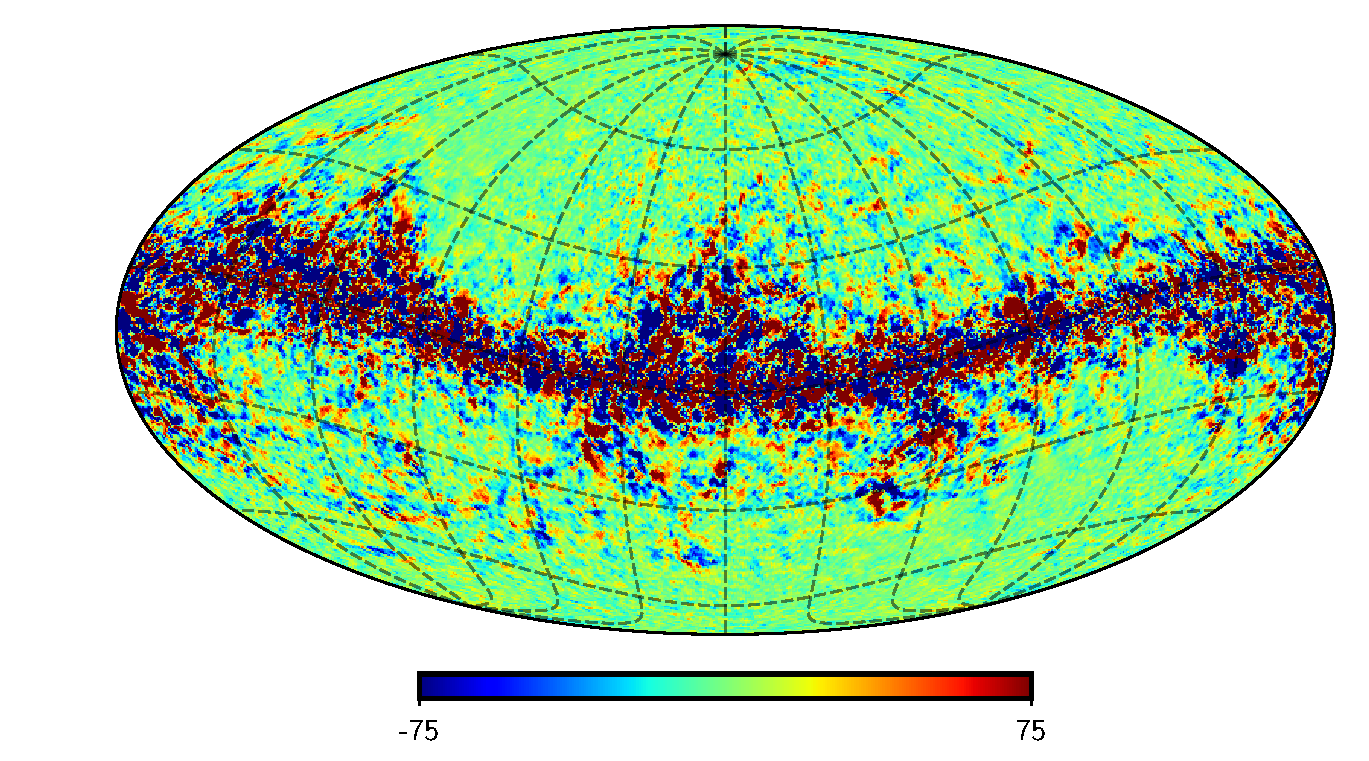
\includegraphics[width=0.49\columnwidth]{353ghz/353ghz-b-mode-realspace_disc7d_apo0d_lmin30_lmax256_nside128.pdf}}
\subfigure[]{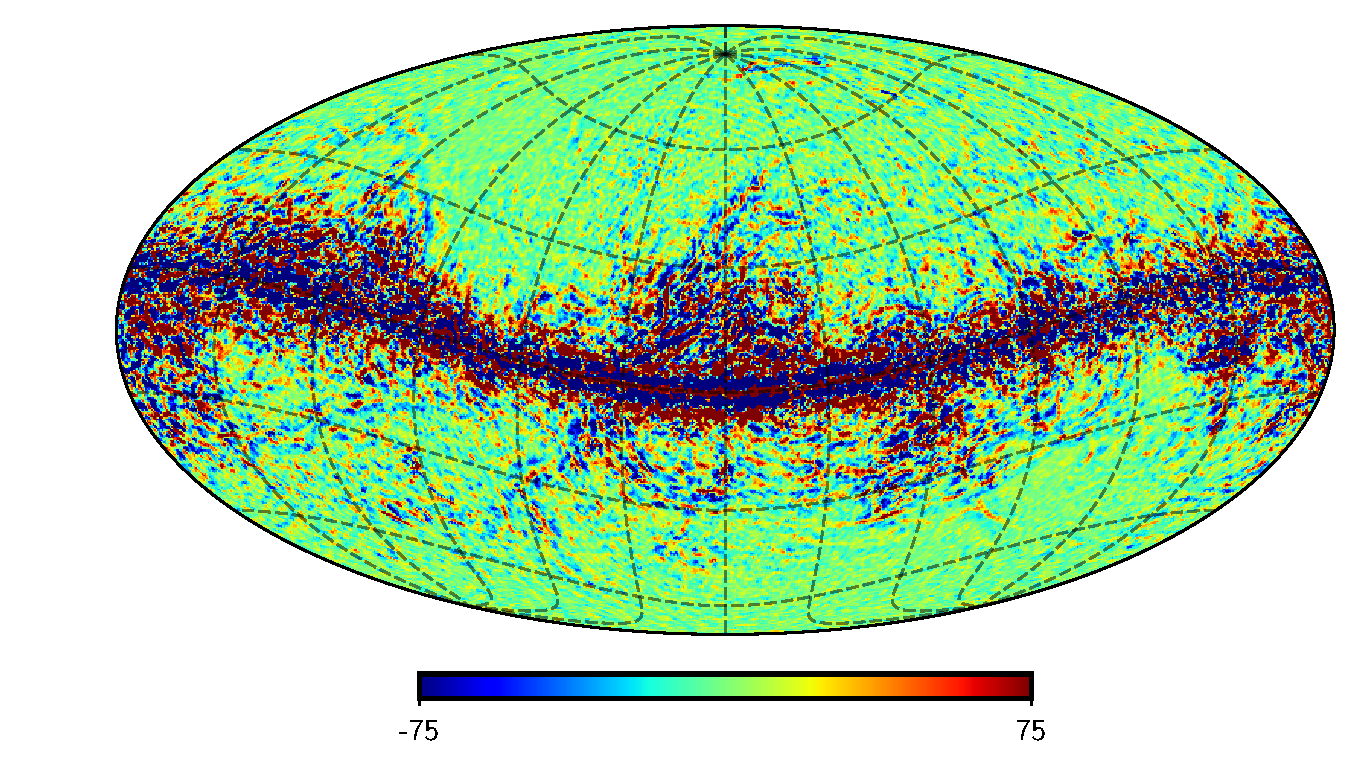
\includegraphics[width=0.49\columnwidth]{353ghz/353ghz-e-mode-realspace_disc7d_apo0d_lmin50_lmax256_nside128.pdf}}
\subfigure[]{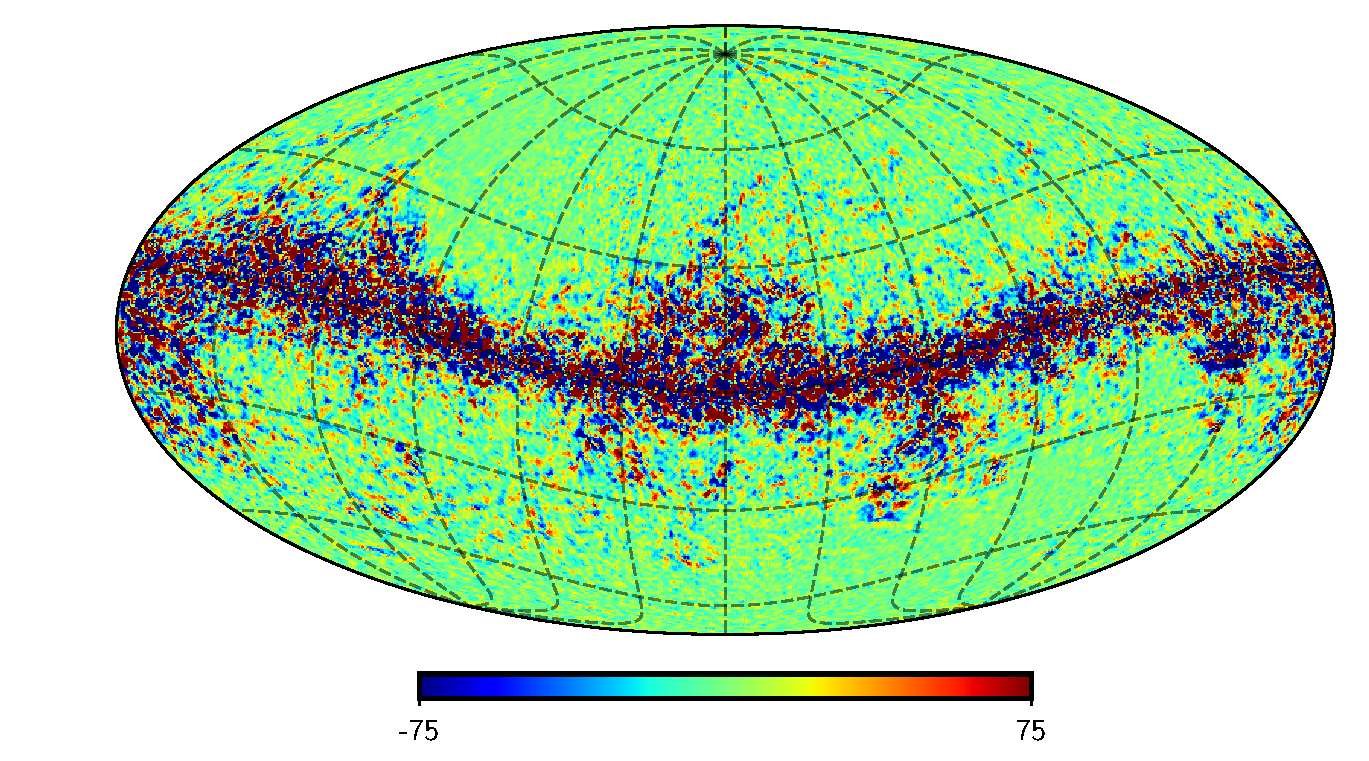
\includegraphics[width=0.49\columnwidth]{353ghz/353ghz-b-mode-realspace_disc7d_apo0d_lmin50_lmax256_nside128.pdf}}
\caption{}
\label{fig:353ghz-eb-maps}
\end{figure}
%
%--------------------------------------------------------
%--------------------------------------------------------

%--------------------------------------------------------
%--------------------------------------------------------
\subsection{Scaling and future prospects}
%
\begin{figure}[!h] 
\centering
\subfigure[]{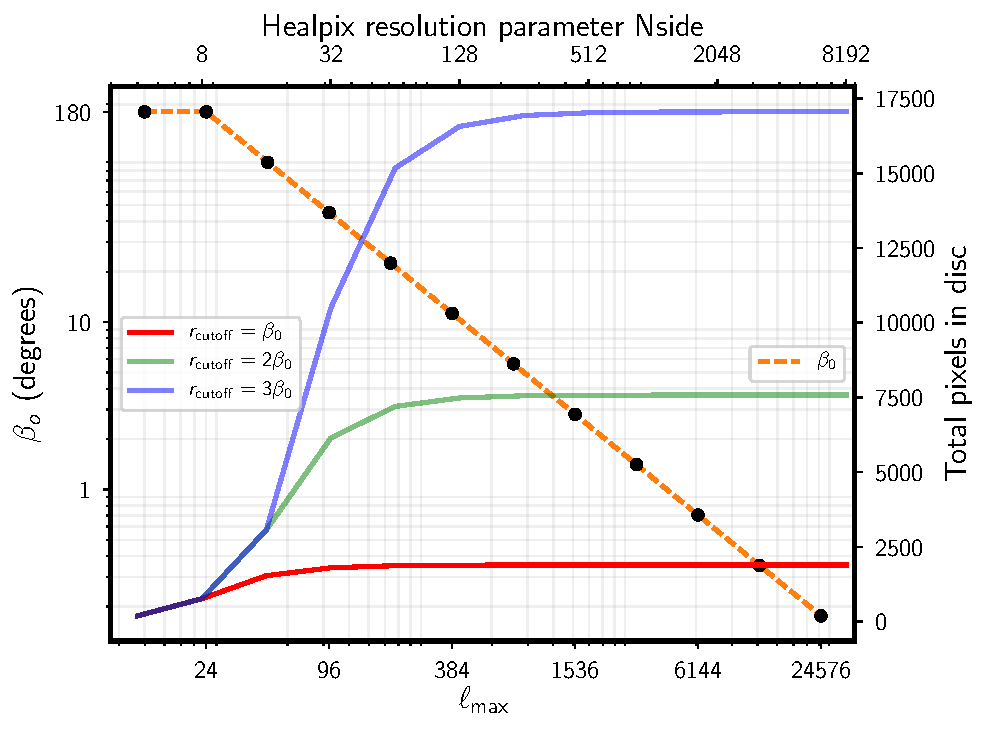
\includegraphics[width=0.8\columnwidth]{supplementary/number_of_disc_pixels.pdf}}
\caption{The red dashed curve depicts the how $\beta_o$ changes as a function of the Healpix resolution parameter Nside assuming that the maximum multipole accessible in the map is given by $\ell_{\rm max} = 3 * Nside$. The blue solid curve depicts the number of surrounding pixel that will need to be accessed to carry out the convolution on Stokes Q \& U maps to infer the value of the scalar fields E \& B at the central pixel.}
\label{fig:disc_rad_healpix_numpix}
\end{figure}
%
%--------------------------------------------------------
%--------------------------------------------------------
